\documentclass{article}
\usepackage{graphicx}
\usepackage{listings}
\begin{document}
\title{Generative Animation}
\author{David E. Shere\\Student ID A11180725\\VIS 40 Section 03}
\maketitle

My project creates a random graph of vertices with seven edges each
and node values containing a state and position.
The position is simply the pixel position for the node to be drawn
and the state is a state of either \emph{Off} or \emph{On}.  \emph{On} states are
accompanied by an integer value representing an \emph{On} "level."
This level is simply a value that is incremented every frame a
vertex is in the \emph{On} state, and decremented when it would be turned off.

The behavior of the nodes themselves is defined by rules for a cellular
automaton where a cell's state is modified based on the states of
their neighbors.  This state
is then used in the drawing function for each frame to determine the
color to draw the node and the node's edges.  Nodes are drawn as circles
and edges as thin lines.  Nodes that have a state of \emph{Off} are drawn
as a very faint blue and nodes that are on vary from a brighter blue to
a brighter red.

Because the nodes are distributed randomly and in a large quantity, the
resulting animation looks chaotic.  The result of the transitions
from blue to red for the nodes as their \emph{On} counter increments is
a shimmering or undulating effect that seems far more organic than
the mathematical process that creates it.
The animation is then something greater than it's parts
and attempts to create the sense of the sublime through a kind of
reverse data visualization; a well defined
collection of information is visualized such that their relationships
are almost entirely lost and the experience as a whole dominates.

\begin{figure}
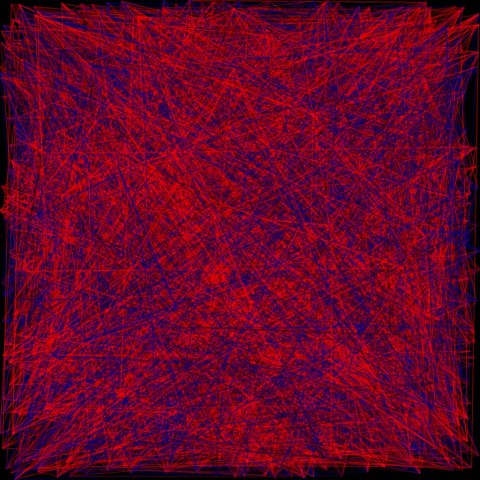
\includegraphics[height=5in]{frame.png}
\caption{Example frame from animation.
Full animation can be seen at http://youtu.be/ZS4ENqjOdxg}
\end{figure}

\newpage
\lstinputlisting[language=haskell,numbers=left]{../graph.hs}
\end{document}
